\chapter{9.Segementierung}

\newcommand{\quo}[1] {
\glqq #1 \grqq
}

Dieses ist die Zerlegung eines Bildes in verschiedene Objekt.\\
Eine einfach methode hierfür ist das \mim{Historgramm thresholding}:
\begin{center}
  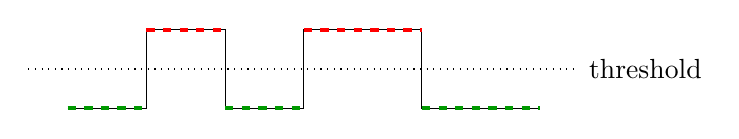
\begin{tikzpicture}
    \draw (1,0) -- (2,0) -- (2,1) -- (3,1) -- (3,0) -- (4,0) -- (4,1) -- (5.5,1) -- (5.5,0) -- (7,0);
    \draw[dotted] (0.5,0.5) -- (7.5,0.5) node[right] {threshold};
    \draw[line width=0.5mm,red,dashed] (2,1) -- (3,1);
    \draw[line width=0.5mm,red,dashed] (4,1) -- (5.5,1);
    \draw[line width=0.5mm,green!60!black,dashed] (1,0) -- (2,0);
    \draw[line width=0.5mm,green!60!black,dashed] (3,0) -- (4,0);
    \draw[line width=0.5mm,green!60!black,dashed] (5.5,0) -- (7,0);
  \end{tikzpicture}
\end{center}
So kann ein Bild in mehrere Objekte zerlegt werden.\\
Hierbei können jedoch diverse Probleme auftreten, die durch preprocessing vermindert werden sollten. Einige der preprocessing methoden sind:
\begin{enumerate}
  \item[-] Entrauschen $\nearrow$ 5.7
  \item[-] Farbraum optimal ausnutzen $\nearrow$ 3.2
  \item[-] \mim{Beleuchtungsausgleich}
\end{enumerate}
Dieser Beleuchtungsausgleich wurde nohc nicht vorher besprochen, das Problem:

\begin{center}
  \begin{tikzpicture}
    \draw (0,0) -- ++(20:1) -- ++(0,1) -- ++(20:1) -- ++(0,-1) -- ++(20:1) -- ++(0,1) -- ++(20:1.5) -- ++(0,-1) -- ++(20:1.5);
    \draw[dotted] (-0.5,1.5) -- (6,1.5) node[right] {threshold??};
  \end{tikzpicture}
\end{center}

Anstatt eines \quo{geraden} Bildes ist das Bild, etwa durch Beleuchtung, \quo{gekippt} und der Ansatz mittels Histogramthresholding würde nicht das gewünschte Ergebniss erzielen.\\

In 2D könnte dies so aus sehen.

\begin{center}
  \begin{tikzpicture}
    \draw[white] (0,0) rectangle node[draw,black] {\includegraphics[scale = 0.2]{images/Bild3plusgrad.png}} (3,3);
    \draw (1.5,3) node[above] {\LARGE $f$};
    \draw (1.5,0) node[below] {gegeben};
    \draw (3.5,1.5) node[] {\LARGE $=$};
    \draw[white] (4,0) rectangle node[draw,black] {\includegraphics[scale = 0.2]{images/Bild3.png}} (7,3);
    \draw (5.5,3) node[above] {\LARGE $u$};
    \draw (5.5,0) node[below] {erwünscht};
    \draw (7.5,1.5) node[] {\LARGE $+$};
    \draw[white] (8,0) rectangle node[draw,black] {\includegraphics[scale = 0.2]{images/Bild3grad.png}} (11,3);
    \draw (9.5,3) node[above] {\LARGE $v$};
    \draw (9.5,0) node[below] {gesucht};
    \draw (11.75,1.5) node[] {\LARGE $\Longleftrightarrow$};
    \draw[white] (12.5,0) rectangle node[draw,black] {\includegraphics[scale = 0.2]{images/Bild3thresh.png}} (15.5,3);
    \draw (14,3) node[above] {};
    \draw (14,0) node[below] {Ergebnis durch thresholding};
  \end{tikzpicture}
\end{center}

Rechts ist das Bild, das durch das Beschreibene Histogramm thresholding dargestellt wurde zu sehen. Methoden um durch preprocessing den gesuchten Gradienten zu entfernen werden im folgenden beschrieben.

\section{Beleuchtungsausgleich}

\begin{enumerate}
  \item[Einfachster Fall:] $v$ konstant. In diesem Fall kann man etwa eine \quo{Leeraufnahme} machen, $v=f$ setzen und dieses $v$ in allen folgenden Aufnahmen subtrahieren.
  \item[Normalfall:] $v$ ändert sich bei Jeder Aufnahme. Hierbei gibt es mehrere Ansätze:
\end{enumerate}

\begin{enumerate}
  \item[a)] \mim{Lineare Regression}: \\
  \begin{minipage}[c]{0.6\linewidth}
          \item[] Wir Unterstellen das der Verlauf \mim{affin-linear} ist, d.h.:
          \[v(x,y) = a x + b y + c\]
          Diese Parameter $a$, $b$, $c$ gilt es nun zu schätzen. 
    \end{minipage}
    \hfill
    \begin{minipage}[c]{0.35\linewidth}
              \begin{center}
        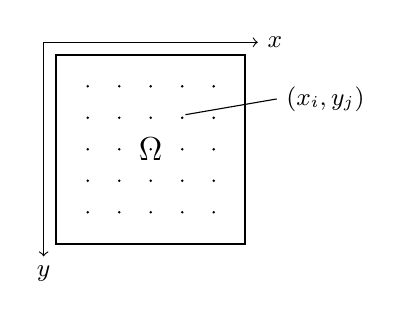
\begin{tikzpicture}[scale=0.8]
          \draw[thick] (0,0) rectangle node[] {\large $\Omega$} (3,3);
          \draw[->] (-0.2,3.2) -- (3.2,3.2) node[right] {\small $x$};
          \draw[->] (-0.2,3.2) -- (-0.2,-0.2) node[below] {\small $y$};
          \foreach \x in {1,...,5}
            \foreach \y in {1,...,5}{
              \draw (\x / 2,\y / 2) node[circle,fill=black,inner sep=0pt] {};
          }
          \draw (2.05,2.05) -- (3.5,2.3) node[right] {\small $(x_i,y_j)$};
        \end{tikzpicture}
      \end{center}
    \end{minipage}
    Dazu soll gelten
    \[\forall (x,y) \in \Omega : ax+by+c \approx f(x,y)\]
    um dieses zu erfüllen wird eine Stichprobe von endlich vielen Punkten $(x_i,y_i)$ aus $\Omega$ gewählt und durch diese ein Gleichungs System gebildet.
    
    \begin{gather*} 
    ax_1+by_1+c \approx f(x_1,y_1)\\
    \vdots \\
    ax_n+by_n+c \approx f(x_n,y_n)
    \end{gather*}
    In Matrix form ergibt sich:
    
    \[\underbrace{\mat{x_1 & y_1 & 1 \\ \vdots & \vdots & \vdots \\ \vdots & \vdots & \vdots \\ \vdots & \vdots & \vdots \\ x_n & y_n & 1}}_{A} \underbrace{\mat{a \\ b \\ c}}_{w} \approx \underbrace{\mat{f(x_1,y_1 \\ \vdots \\ \vdots \\ \vdots \\ f(x_n,y_n)}}_{z}\]
    Die optimale Lösung dieses Problems kann über die \mim{Normalengleichung} berechnet werden.
    
    \[A^T A w = A^T z\]
    
    Dauraus erhält man $w$, somit auch $a$, $b$, $c$ und schlussendlich $v \Rightarrow u = f-v$.\\
    Anschließend wird noch ein Histogram stretching durchgeführt um das finale Bild zu erhalten.
    
    \item[b)] \mim{Polynomiale Regression}:
    Ähnlich zur linearen Regression nun wird hierbei keine affin-lineare Funktion, sondern ein polynom genutzt. Für ein Polynom zwieten gerades kann etwa die Funktion
    \[v(x,y) = ax^2 by^2 cxy+ dx +ey +f\]
    gewählt werden. Wieder entsteht ein Gleichungssytem:
    
    \[\underbrace{\mat{x_1^2 & y_1^2 & x_1y_1 & x_1 & y_1 & 1 \\ \vdots & \vdots & \vdots & \vdots & \vdots & \vdots \\ \vdots & \vdots & \vdots & \vdots & \vdots & \vdots \\ \vdots & \vdots & \vdots & \vdots & \vdots & \vdots \\ x_n^2 & y_n^2 & x_ny_n & x_n & y_n & 1}}_{A} \underbrace{\mat{a \\ b \\ c \\ d \\e \\ f}}_{w} \approx \underbrace{\mat{f(x_1,y_1 \\ \vdots \\ \vdots \\ \vdots \\ f(x_n,y_n)}}_{z}\]

  \item[c)] \mim{Trigonometrisches Polynom}
  Hierbei wird $v$ in den niedrigfrequenten Anteilen von $f$ gesucht.
  
  \begin{center}
    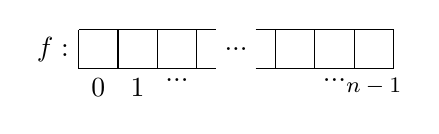
\begin{tikzpicture}
      \draw (0,0.25) node[left] {$f:$};
      \draw[step = 0.5] (0,0) grid (1.75,0.5);
      \draw (2,0.25) node[] {$...$};
      \draw[step = 0.5] (2.25,0) grid (4,0.5);
      \draw (0.25,0) node[below] {$0$};
      \draw (0.75,0) node[below] {$1$};
      \draw (1.25,0) node[below] {$...$};
      \draw (3.25,0) node[below] {$...$};
      \draw (3.75,0) node[below] {\footnotesize $n-1$};
    \end{tikzpicture}
  \end{center}
  
  Es ergibt sich $\hat f$:
  
  \[\hat f_k = \sum_{m=0}^{n-1} f_k \bigl(\underbrace{e^{- i 2 \pi \frac{k}{n}}}_{w_k}\bigr)^m \quad , \ k= 0,1,...,n-1\]
  
  Mittels der FFT (Fast Fourier Transformation) ergibt sich $\hat f$ zu:

  \begin{center}
    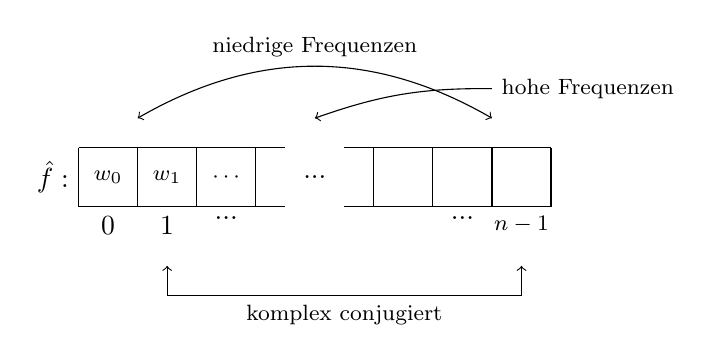
\begin{tikzpicture}[scale=1.5]
      \draw (0,0.25) node[left] {$\hat f:$};
      \draw[step = 0.5] (0,0) grid (1.75,0.5);
      \draw (2,0.25) node[] {$...$};
      \draw[step = 0.5] (2.25,0) grid (4,0.5);
      \draw (0.25,0) node[below] {$0$};
      \draw (0.75,0) node[below] {$1$};
      \draw (0.25,0.25) node[] {\footnotesize $w_0$};
      \draw (0.75,0.25) node[] {\footnotesize$w_1$};
      \draw (1.25,0) node[below] {$...$};
      \draw (3.25,0) node[below] {$...$};
      \draw (1.25,0.25) node[] {\footnotesize$\cdots$};
      \draw (3.75,0) node[below] {\footnotesize $n-1$};
      \draw[<->] (0.75,-0.5) -- (0.75,-0.75) -- node[below] {\footnotesize komplex conjugiert} (3.75,-0.75) -- (3.75,-0.5);
      \draw[<->] (0.5, 0.75) to[bend left] node [above] {\footnotesize niedrige Frequenzen} (3.5,0.75);
      \draw[<-] (2,0.75) to[bend left=10] (3.5,1) node[right] {\footnotesize hohe Frequenzen};
    \end{tikzpicture}
  \end{center}
  Durch entfernen dieser niedrigen Frequenzen ergibt sich $u$.
Ähnliches funktioniert auch in 2D:

    \begin{center}
    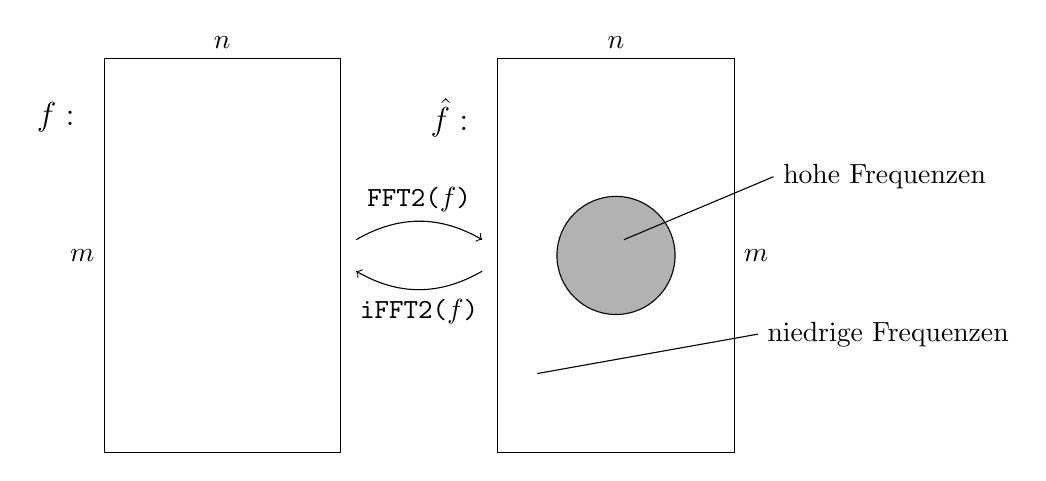
\begin{tikzpicture}[scale=1]
      \draw (0,0) rectangle (3,5);
      \draw (1.5,5) node[above] {$n$};
      \draw (0,2.5) node[left] {$m$};
      \draw (-0.25,4.25) node[left] {\large $f:$};
      \draw[->] (3.2,2.7) to[bend left] node[above] {\tt{FFT2($f$)}} (4.8,2.7);
      \draw[<-] (3.2,2.3) to[bend right] node[below] {\tt{iFFT2($f$)}} (4.8,2.3);
      \draw (5,0) rectangle (8,5);
      \draw (6.5,5) node[above] {$n$};
      \draw (8,2.5) node[right] {$m$};
      \draw (4.75,4.25) node[left] {\large $\hat f:$};
      \draw[fill = black!30] (6.5,2.5) circle (0.75);
      \draw (6.6,2.7) -- (8.5,3.5) node[right] {hohe Frequenzen};
      \draw (5.5,1) -- (8.3,1.5) node[right] {niedrige Frequenzen};
    \end{tikzpicture}
  \end{center}
\end{enumerate}
